\chapter{Research}\label{research}
%TODO Mention RQ, problem statement
The aim of this paper is to examine the effect of reducing the dimensionality of the state-space in reinforcement learning (RL). In this section we will discuss the our research and its results. We will start by detailing our method in section \ref{research-method}; here we will explain the environment we used for our experiments, as well as the experiments that we ran. After this, we will show and discuss the results from these experiments in section \ref{research-results}. The discussion of the results will include an examination of how the different state-space reduction methods led to their results.


\section{Method}\label{research-method}
In this section we will explain our method: how we researched the effect of state-space dimensionality reduction on an RL agent. Before going into the details of the different experiments that we ran in section \ref{research-exp}, we will first look at the environment in which we ran the experiments in section \ref{research-env}.

\subsection{Environment: Starcraft II}\label{research-env}
For our experiments we used the \emph{StarCraft II} environment by \emph{Blizzard}\cite{blizzard}. StarCraft II is a real-time strategy game, which has been used in RL research after the introduction of a learning environment created in collaboration with \emph{DeepMind}, called \emph{SC2LE} and a corresponding Python component called \emph{PySC2}\cite{pysc2}.

In particular we are using a PySC2 minigame called \emph{MoveToBeacon}. This minigame simplifies the StarCraft II game. Here, the RL agent must select an army unit and move it to a given beacon. To simplify our RL agent, selecting the army unit is implemented as a script, thereby focusing our research on moving the army unit to the beacon. A screenshot of the game is given in figure \ref{fig:pysc2_SS}. 

\begin{figure}[h]
    \centering
    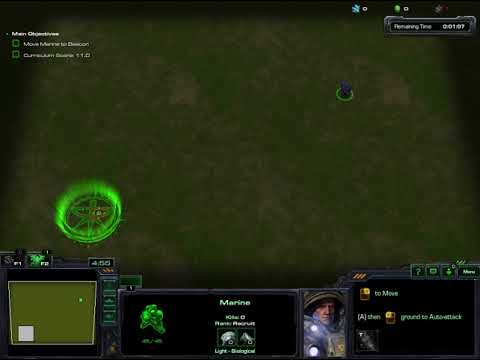
\includegraphics[width=0.75\textwidth]{pysc2_SS}
    \caption{Screenshot of the minigame \emph{MoveToBeacon} in \emph{StarCraft II}.}
    \label{fig:pysc2_SS}
\end{figure}

An \emph{observation} received by the agent in this minigame is given by a $32 x 32$ grid, representing the entire state of the game, \todo{Is this correct? Or are there actually perhaps only 3 features or something?} giving a total of \emph{$1024$ features}. Each cell in the grid represents a tile in the game. It can have one of three values: a 0 denoting an empty tile, a 1 denoting the army unit controlled by the agent, or a 5 denoting the beacon. The beacon comprises more than one tile, namely a total of $21$ tiles; it comprises five adjecent rows, where the first comprises three adjecent columns, followed by three rows of five columns, followed by a row of three columns. Because of this, the beacon has $27 \time 27$ places where it could be, with the army unit having $1003$ tiles left to be. This gives \todo{Is this a correct usage of state-space?} a total state-space of $32 x 32 x 3$ with a cardinality of $27 \time 27 \times 1003 = 731.187$. An example of such a state observation can be seen in figure \ref{fig:state_example}.

\begin{figure}[h]
    \centering
    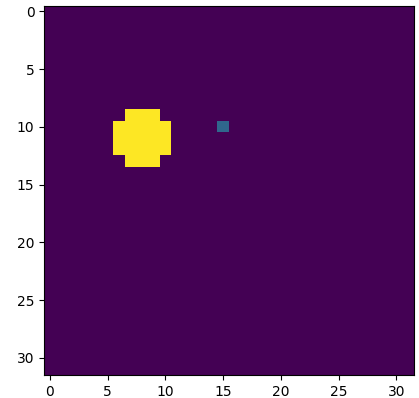
\includegraphics[width=0.75\textwidth]{AE_State_original}
    \caption{A state observation received by the RL agent, for the StarCraft II minigame MoveToBeacon. The yellow cells represent one beacon; the blue cell represents the army unit controlled by the player; all other cells are empty.}
    \label{fig:state_example}
\end{figure}

An \emph{action} taken by the agent is given by an $(x,y)$ coordinate with $x,y \in \{0 .. 31\}$. This denotes the (indices of the) cell in the grid that the army unit will move to.

Lastly, an \emph{episode} takes $120$ seconds. The goal is to move the army unit to the beacon as often as possible in this time limit, each time adding $1$ point to the episode score. At the start of each episode, the beacon and army unit are placed randomly. Whenever the army unit reaches the beacon, only the beacon will be relocated randomly.  

\subsection{Experiments}\label{research-exp}
Welke experiments/vergelijkingen gedaan + setup

\begin{itemize}
\item Base agent
\item PCA agent
\item Pretrained AE agent
\item Online trained AE agent
\item DeepMDP
\end{itemize}


\section{Results}\label{research-results}
sectie opzet
\subsection{Research results}
Resultaten van de verschillende agents

\subsection{Discussion}
Resultaten van AE analyse

